\documentclass[amssymb,twocolumn,prd,nofootinbib,showpacs]{revtex4-1}

\usepackage{graphicx}  % needed for figures
\usepackage{dcolumn}   % needed for some tables}
%\usepackage[style=authoryear,backend=biber]{biblatex}
\usepackage{bm}        % for math
\usepackage{amsmath,amssymb}
%\usepackage{natbib}
\usepackage{hyperref}
\usepackage{color}
\definecolor{purple}{rgb}{0.58,0.0,0.83}
\usepackage{caption}
\usepackage[toc,page]{appendix}
\usepackage{bm}        % for math
\usepackage{amsmath,amssymb}
\usepackage{hyperref}
\usepackage{color}
\usepackage{braket}
\definecolor{purple}{rgb}{0.58,0.0,0.83}
\usepackage{caption}
\usepackage[toc,page]{appendix}
\usepackage{subcaption}
\newcommand{\jav}[1]{\textcolor{red}{(jav: #1)}}
\newcommand{\lp}[1]{\textcolor{blue}{(lp: #1)}}


\begin{document}

\title{On the two field inflationary models and constraints for ultra-light scalar field dark matter spectators during inflation}
\author{Luis E. Padilla}  
\email{epadilla@fis.cinvestav.mx}
\affiliation{Departamento de F\'isica, Centro de Investigaci\'on y de Estudios Avanzados del IPN, 
A.P. 14-740, 07000 M\'exico D.F.,  M\'exico.}
   \author{J. Alberto V\'azquez}  
\email{javazquez@icf.unam.mx}
\affiliation{Instituto de ciencias f\'isicas, Universidad Nacional Aut\'onoma de M\'exico, sede Cuernavaca, 
Morelos, M\'exico}
\author{Tonatiuh Matos}  
\affiliation{Departamento de F\'isica, Centro de Investigaci\'on y de Estudios Avanzados del IPN, A.P. 14-740, 
07000 M\'exico D.F.,  M\'exico.}
   \author{Gabriel Germ\'an}  
\affiliation{Instituto de ciencias f\'isicas, Universidad Nacional Aut\'onoma de M\'exico, sede Cuernavaca, 
Morelos, M\'exico}

\date{\today}

\begin{abstract}
Cosmological inflation is nowadays the most accepted mechanism to explain the  primordial seeds 
that led to  the structure formation observed in the Universe. Current observations are in well agreement 
to initial adiabatic conditions, which implies that  single-scalar-field inflation may be enough to describe 
the early Universe. 
%
However, there are several scenarios where more than a single field could be relevant during inflation. 
The simplest situation is where the so-called spectator is present. 
In this paper we initially review the formalism for two field inflationary models and then to apply it to two different 
spectator scenarios. Firstly, to the possibility that an ultra-light scalar field dark matter coexist with the inflaton, 
where such ultra-light field could be auto-interacting or only massive. Secondly, to the curvaton scenario.
In both cases we provide a comparison to current cosmological data.    
\\
\jav{cuesta un poco de trabajo identificar que ya se obtuvo en otros articulos y que se obtiene aqui. 
Tratar de poner enfasis en lo nuevo.}
\jav{Hay muchos 'consider', 'scalar field', 'start', 'scenario', 'notice', 'in this way', 'we can', 'using', 
agregar sinonimos o cambiar frases.}
\jav{Acomodar secciones, subsecciones, subsubsubsecciones}
\jav{obtienes constricciones en terminos de $r$, y no vuelves a mencionar $n_T$. mencionar algo sobre este numero.}
\end{abstract}
\pacs{????}
\begin{keywords}
a Inflation  --  Isocurvature  --  Scalar field -- Dark Matter
\end{keywords}

\maketitle


%%%=========================================================================%%%
\section{Introduction}
\label{introduction}
%%%=========================================================================%%%

It is well accepted that the primordial seeds of the structure formation in the Universe were generated by quantum 
fluctuations provided by a scalar field (SF) during an inflationary era. 
The simplest scenario where density perturbations are carried out by a single inflaton is quite preferred 
since the initial perturbations are nearly adiabatic \cite{const1,const2,planck}. However the presence of any light field, other than the inflaton, could also fluctuate during inflation and contribute to the primordial desity perturbations. Of special interest is the possibility that this extra SF can be used as a dark 
matter component (DM). This scenario is usually known as scalar field dark matter (SFDM) and propose that DM is composed of bosonic excitations of an ultra-light SF. The tipical mass of this model is around $m\sim 10^{-22}eV/c^2$, which might include self-interaction.
%

The idea of scalar fields as DM was initially introduced by \cite{SF1} and since then rediscovered 
using different names, for instance Scalar Field Dark Matter  (SFDM)  \cite{SF2},  Fuzzy  DM  \cite{SF3}, 
Wave DM \cite{SF4,SF5}, Bose-Einstein Condensate DM \cite{SF6} or Ultra-light Axion DM \cite{SF7,SF8}, 
amongst many others. 
%
The purpose of this field is to resolve the apparent conflict, with observations, that exhibits the
cold dark matter (CDM) formed of weakly-interacting massive particles (WIMPS) \cite{LCDM1,LCDM2}. 
%was proposed due to the fact that the preferable model, which considers the DM as cold and assumes to be formed 
%of weakly-interacting massive particles (WIMPS) \cite{LCDM1,LCDM2}, is in apparent conflict with observations on 
Some of these weaknesses may appear at small-scales within galaxies, e.g. cuspy halo density profiles, overproduction of 
satellite dwarfs within the Local Group and many others, see for example \cite{problem1,problem2,problem3,problem4,problem5}). 
Since then, the SFDM model has been successfully tested by different observations;  
for a review on ultra-light SFDM see \cite{SF9,SF10,SF11,SF12}. 

This paper is organized as follows: First, in section \ref{Generalities} we review the basics about the inflationary scenario. 
Then in section \ref{experimentos} we present the basic inflationary observables used to constraint our models. 
Once the mathematical background and the observational constrictions are given, in section \ref{simplest} we 
analize two different models. 
First, we assume a massive SFDM spectator during inflation. We provide some limits for the SFDM mass using isocurvature constrictions and comparing them with the actual constraints given by astrophysical and cosmological observations. 
 Then we consider a self-interacting term for the SFDM. We constraint their parameters using isocurvature perturbations and we compare our results with cosmological and astrophysical observations. Finally in section \ref{conclusions} our conclusions are given.      

%%%=========================================================================%%%
\section{Generalities for two field inflationary models}\label{Generalities}
%%%=========================================================================%%%


In this section we will review in a very short way the iflationary process for spectator-like SFs during iflation following \cite{twofields} (see also \lp{Referenciar nuestro paper} for a more recent review). In this paper we work using natural units ($\hbar=c=1$).

%
A  SF $\phi_i$ living  during  the  inflationary  era  is  tought
to acquire quantum fluctuations with a primordial power
spectrum meassured at Hubble exit as
\begin{equation}\label{eq1}
P_{\phi_i}\simeq\left(\frac{H_*}{2\pi}\right)^2
\end{equation}
Here  and  for  the  rest  of  this  work  quantities  with subindex $*$ means quantities measured at Hubble exit. 

If during the inflationary era there are more than one SF,  it  is  common  to  work  in  a  rotating  basis,  defining
the \textit{adiabatic field} $\sigma$ parallel  to  the  trajectory  in  field space and the \textit{entropy fields} $s_i$ perpendicular to it. If the background trajectory is a stright-line and evolves in the direction of the field that causes the inflationary process, the scenario is called the \textit{inflaton scenario} (IS). In this scenario  the  quantum  fluctuations $\delta\sigma$ of  the  adiabatic field  and $\delta s_i$,  wich  are  also  called  \textit{spectator fields}, are frozen at Hubble exit\footnote{If the trayectory is curved in field-space, the entropy and adiabatic perturbations are correlated at Hubble exit and the perturbations continue evolving until inflation ends \cite{twofields}} and start evolving until they re-enter to the horizon. We consider the case when there is only one extra SF in addition to the inflaton. In this way the primordial power spectrum is given by
\begin{equation}\label{eq2}
P_{\sigma^*}(k)=P_{s}^*(k)\simeq\left(\frac{H_*}{2\pi}\right)^2,
\end{equation}

On the other hand, the curvature and isocurvature perturbations are defined as
%
\begin{equation}\label{RS}
R\equiv\frac{H}{\dot\sigma}\delta \sigma, \ \ \ S=\frac{H}{\dot \sigma}\delta s.
\end{equation}
Then, the final power spectra, at the beginning of the radiation-domination era, are thus
%
\begin{equation}\label{PRf}
P_R=P_S\simeq P|_*,
\end{equation}
%
where at linear order in slow-roll parameters
%
\begin{equation}
P|_*=\frac{1}{2\epsilon}\left(\frac{H_*}{2\pi M_{pl}}\right)^2,
\end{equation}
%
with $M_{pl}=1.221\times 10^{19}GeV$ the Planck mass.\\

%%%-------------------------------------------------------------------------------------------%%%
\textit{Gravitational waves.-}
%%%-------------------------------------------------------------------------------------------%%%
Given  the  fact  that  scalar  and tensor  perturbations  are  decoupled  at  linear  order,  the amplitude  of the  gravitational  waves  spectrum and  the tensor-to-scalar ratio $r$ in the IS is the same than in the case where there are not extra spectator fields during the inflationary process.

We  can  see  then  that  the  incorporation  of  this  new fields during the IS will produce only isocurvature perturbations.  Such perturbations can be used to constraint the free parameters of our SFDM models as we will see later.
%%%=========================================================================%%%
\section{Constraints on inflationary parameters}\label{experimentos}
%%%=========================================================================%%%

In the standard approximation the inflationary observables are given by the tensor to scalar ratio $r$, 
the spectral index for adiabatic perturbations $n_R$ and the amplitude for adiabatic perturbations $A_r^2$.  
The constraints of these parameters are quoted at the pivot scale $k_0=0.05 Mpc^{-1}$ 
by \cite{const1,const2,planck,const3,const4,const5}\lp{Agregar referencia del nuevo Planck}
%
\begin{subequations}
\begin{equation}\label{amplitude}
A_r^2(k_0)=(2.215^{+0.032}_{-0.079})\times 10^{-9}, \ \ \ \text{at $68\%$ CL},
\end{equation}
\begin{equation}
r_{k_0}<0.064 \ \ \ \text{at $95\%$ CL},
\end{equation}
\begin{equation}\label{n_R}
n_R(k_0)=0.968 \pm 0.006.
\end{equation}
\end{subequations}
%
Using these measurements we are able to constrain the value of the Hubble expansion rate during 
inflation $H_*$ as \cite{H1,H2}
%
\begin{equation}\label{Hinf}
r = 1.6\times 10^{-5}\left(\frac{H_{inf}}{10^{12}GeV}\right)^2.
\end{equation}

As we have seen beforehand, if more than one SF is present during inflation we will obtain isocurvature 
perturbations generated by extra scalar fields perpendicular to the trajectory on field space. 
%
Parameterizing the isocurvature power spectrum for dark matter in terms of the curvature power as
%
\begin{equation}\label{isoCDM}
P_{DM}(k) = \frac{\beta_{iso}(k)}{1-\beta_{iso}(k)}P_R(k),
\end{equation}
%
where $P_{DM}=\braket{\delta \rho_{DM*}/\rho_{DM}}$, $\delta\rho_{DM}$ are the isocurvature 
perturbations for the dark matter ($DM$) generated by extra scalar fields during inflation and $\rho_{DM}$ 
is the initial condition of DM. 
The uncorrelated scale-invariant DM isocurvature is constrained by Planck data \cite{const1,const2} 
at pivot scale $k_0$ as
%
\begin{equation}\label{betaiso}
\beta_{iso}(k_0)<0.038 \ \ \ \text{at $95\%$ CL}.
\end{equation}
%
Notice that isocurvature perturbations can be used to constraint the inflationary scale, 
just by combining equations \eqref{Hinf}, \eqref{isoCDM} and \eqref{betaiso}.
%
%
%
%%%=========================================================================%%%
\section{CONSTRAINING MASSIVE AND
SELF-INTERACTING ULTRA-LIGHT SFDM
MODELS}\label{simplest}
%%%=========================================================================%%%
In this section we consider the possibility that an ultra-light  SFDM  candidate  coexist  with  the  inflaton  during the inflationary era.  We require that the SFDM candidate be a stable spectator field with negligible classical dynamics and energy density.  We can obtain such scenario by considering the IS, i.e.  that the trajectory in the field space evolves in the inflaton direction $\phi$ whereas the direction perpendicular to the trajectory corresponds to the SFDM $\psi$. Notice that it is necessary ( \jav{pq necesario? o de donde se ve?}\lp{Se ve de pedir que evolucione m\'as lento que el inflat\'on, como lo ped\'i arriba)} that our dark matter candidate evolves much slower than the inflaton and its density be smaller than the associated to the inflaton. 

As we mentioned it is possible to constraint the free parameters of our model when isocurvature perturbations are considered.  For this reason in the next subsections we review the cosmological history that a massive and a self-interacting scalar field should have gone through the evolution  of  the  Universe,  since  it  will  be  necessary  to match the values of the field at the present with the field during the inflationary era in order to take into acount isocurvature constrictions. We also consider the different cosmological  and  astrophysical  constraints  obtained  for each SFDM model in order to compare our results.  Let us now explain the way it is obtained. 

First at all let us remember the basics about SFs. The dynamical evolution of any SF is governed by the Klein-Gordon (KG) equation
\begin{equation}
\Box\Psi-2\frac{dV}{d|\Psi|^2}\Psi=0.
\end{equation}
When a SF is complex it is convenient to use a Madelung transformation \cite{madelung}
\begin{equation}
\psi = \eta \exp[i\theta],
\end{equation}
%
where $\eta\equiv |\psi|$ is the magnitude of field $\psi$ and $\theta$ its phase. With this new descomposition the KG equation is separated in its real and imaginary components as
%
\begin{subequations}\label{KESFDM}
\begin{equation}\label{KGe1}
\ddot\eta+3H\dot\eta+2\frac{dV}{d|\psi|^2}\eta-\omega^2\eta= 0,
\end{equation}
\begin{equation}\label{KGe2}
\dot\omega \eta + (2\dot\eta+3H\eta)\omega=0,
\end{equation}
\end{subequations}
%
where $\omega = \dot \theta$. Equation \eqref{KGe2} can be exactly integrated obtaining 
%
\begin{equation}
a^3\eta^2\omega=Q,
\end{equation}
%
where $Q$ is a charge of the SF related with the total number of particles \cite{SFphi42,charge1,SFphi41,charge3,charge4}. Plugging this last equation into \eqref{KGe1} we obtain
the radial component of the scalar field follows
%
\begin{equation}\label{KGe3}
\ddot\eta+3H\dot\eta+M^2\eta-\frac{Q^2}{\eta^3}= 0.
\end{equation}
%
The term containing $Q$ is obtained by the complex nature of the SF \cite{SFphi42} and can be interpreted 
as a ``centrifugal force" \cite{charge4}; $M^2\equiv 2(dV/d|\psi|^2)$ can be seen as an effective mass term 
of the scalar field. Notice that if we consider $\Psi$ as the SFDM and we take $Q^2/\eta^3\ll 1$ assuming the SFDM candidate fulfills the slow-roll condition during inflation, then the field $\eta$ will remain frozen at value $\eta_i$ until $H\sim M$, where here and for the rest of this work subindex $i$ means values obtained right after inflaiton ends. Then, when $H\sim M$ will start evolving depending on the effective mass term. Notice that in order to obtain a slow-roll behavior of the SFDM it is neccesary that $|\theta|\ll 1$ as it is explained in \lp{Referencia paper Abril} \jav{pq, si es solo una fase?}\lp{Seg\'un yo por lo que dice la footnota}\footnote{In fact the inflationary behavior is an attractor solution of the KG equation for a real field in the limit when $M^2\ll H^2$ \cite{atractorinf1,atractorinf2}.
 In this limit the typical dynamics of a real SF is a stiff-like epoch, followed by an inflationary-like era. }. On the other hand if $\Psi$ is the inflaton $\phi$, it is usually considered as a real field. Then in this case $\theta=Q=0$.
 
In this work we consider only situations where the general potential can be descomposed as $V(\phi,\psi)=V_{inf}(\phi)+V_{SFDM}(|\psi|^2)$.

%%%-------------------------------------------------------------------------------------------%%%
%\begin{center}
\subsection{Real ultra-light SFDM candidate}
%\end{center}
%%%-------------------------------------------------------------------------------------------%%%
\subsubsection{Cosmological history for a real ultra-light SFDM particle}
The  possibility  that  an  ultra-light  SFDM  candidate could  coexist  with  the  inflaton  has  been  recently  studied in \cite{SFrev2} considering a full potential of the form
\begin{equation}\label{potential_massive}
V(\phi,|\psi|^2)=V(\phi)+\frac{1}{2}m^2\psi^2.
\end{equation}
%
and by fixing $Q=0$ for the SFDM in Eq. \eqref{KGe3}. Such study was obtained by considering the SFDM as an axion-like particle. However their results can be extrapolated for whichever massive SFDM. For this particular case we observe that  $M^2=m^2$. As mentioned above when $H\gg m^2$ the term with $m^2$ 
in equation \eqref{KGe1} can be neglected. Since we considered the field is slowly rolling during the inflationary era, 
we can neglect the second derivatives in \eqref{KGe1}, then the field $\psi$ remains frozen at its initial value by 
Hubble dragging during the early universe \cite{curvatonatractor}. 
%
Then, when approaches the condition $m\sim H$ the SFDM starts evolving and oscillates as a massive field. 
During its oscillation phase the dependence of $\psi$ respect to $a$ is $\psi\sim 1/a^{3/2}$, while its density 
behaves as $\rho_{\psi}\sim 1/a^3$  \cite{SFphi41,SFphi42}. In this way we can write the scalar density 
of our field as \jav{$\psi_i$ se confunde con condicion inicial.}\lp{De hecho es la condici ́on inicial que sale de inflaci ́on.  Osease, de inflaci ́on tiene ese valor y empieza a evolucionar cuando comienzan las oscilaciones del campo.}

\begin{equation}\label{rhosfdm}
\rho_\psi = \left\lbrace\begin{array}{ll}
\frac{1}{2}m^2\psi_i^2 & \text{when }H\gg m, \\
\frac{1}{2}m^2\psi_i^2\left(\frac{a_{osc}}{a}\right)^3 & \text{when }H\ll m.
\end{array}\right .
\end{equation}

The typical mass for a SFDM candidate is around $10^{-22} eV$. This implies that the field started oscillating during the radiation-dominated Universe. During this period the Hubble parameter evolves in terms of the scale factor as $H\propto a^{-2}$, and the KG equation \eqref{KGe1} can be solved exactly in terms of $a$. In Ref. \cite{SFrev2} it was obtained the initial conditions for the massive case by considering an evolution of the form \eqref{rhosfdm} and by taking into account that the entropy of the Universe is conserved. Considering that the totallity of the dark matter is composed of SFDM particles they obtain
\begin{equation}\label{phi_im2}
\psi_i^2\simeq\frac{10^{34}GeV^2}{0.6}\left(\frac{g_{*osc}}{3.36}\right)^{-3/4}\left(\frac{g_{s*osc}}{3.91}\right)\left(\frac{m}{10^{-22}eV}\right)^{-1/2}.
\end{equation}
%
Here $g_{*osc}$ and $g_{s*osc}$ are the effective degrees of freedom associated with total particles and entropy at SFDM oscilations. For the particular case of an ultra-light SFDM which starts its oscillations in the radiation-dominated Universe $g_{∗osc}= 3.36$ and $g_{s∗osc}= 3.91$

%%%-------------------------------------------------------------------------------------------%%%
\subsubsection{Constraining isocurvature perturbations for a massive SFDM model}
%%%-------------------------------------------------------------------------------------------%%%

For this case we demand the 
energy density contribution of the SFDM being small during inflation (DM dominates at radiation-matter equality) 
and hence it is necessary that 
%
\begin{equation}
\frac{m^2}{2} < \frac{V(\phi)}{\psi_i^2}\simeq \frac{H^2_{*}M_p^2}{\psi_i^2},
\end{equation}
%
where during inflation our field remains frozen  at value $\psi_i$. 
Notice that for an ultra-light SFDM candidate  ($m\sim 10^{-22}eV$) the above expression is fulfilled for most of the 
initial conditions given by $\psi_i$. 
%
On the other hand we can constraint isocurvature perturbations generated by a SFDM using Eqn. \eqref{isoCDM} or equivalently \eqref{betaiso}. The way it is done was studied in ref \cite{SFrev2} by noticing  that  we  can  re-express  the  primordial spectrum as $\delta\rho_\psi/\rho_\psi = 2\delta\psi/\psi_i$ (since  from  Eq.   \eqref{rhosfdm} we have $\rho_{SFDM}\propto \psi^2$) which implies that $P_{SFDM}=4P_{\psi}/\psi_i^2$, where $P_\psi$ is given by equation \eqref{eq1} or  \eqref{eq2} and $\psi_i$ by equation \eqref{phi_im2}, and then compare it with $P_{DM}$ from equation \eqref{isoCDM}.  When such comparison is done they finally obtain the result
\begin{equation}\label{constm}
\frac{m}{10^{-22}\ eV}<\left(\frac{2\times 10^{-4}}{r}\right)^2.
\end{equation}


The above relation for the mass parameter must be in agreement with the cosmological and astrophysical constrictions  obtained by this model. For example when the model is tested at galactic levels, by considering that the ground state of the self-gravitating BEC corresponds to the minimum DM halo, it is obtained a mass $m\simeq 2.92\times 10^{-22}eV$ \cite{massconst1,SFphi42}; if on the other hand the massive model is tested at cosmological levels considering big bang nucleosynthesis (BBN) and CMB, it is obtained that the model must be self-interacting (see \cite{SFphi41,SFphi42}). When the BBN contriction is ignored it is obtained that $m$ must fulfill $m>7.38\times10^{-19}eV$ which is clearly in disagreement with the constraints given by galactic scales. 

 Figure \ref{constraintsSFDM} displays the last paragraph on a $m\ vs\ r$ plane. The dot-dashed black line corresponds to the value when in Eq. \eqref{constm} we have an equality instead of the inequality sign. The green region is the one that fulfills the relation \eqref{constm} and then it is allowed by isocurvature constrictions. The orange region is allowed by iscorvature and CMB (ignoring by the momment BBN), while the dot-dashed red line corresponds with astrophysical and isocurvature. As we notice, in order to fulfill CMB observations with the lighter SFDM candidate ($m\simeq 7.38\times 10^{-19}eV$) we should no detect gravitational waves until $r\lesssim 2.33\times 10^{-6}$, while if we required that astrophysical observations are fulfilled it should be neccesary the no dectectability of gravitational waves until $r\lesssim 10^{-4}$. These constraints are important given that \cite{laldm} demonstrated that an ultra-light axion-like dark matter candidate must be presented during inflation. \jav{como? no es lo que estamos buscando mostrar nosotros?}\lp{No,  nosotros  estamos  partiendo
de  la  premisa  de  qu\'e  pasar\'ia  si  el  campo  escalar  vivi\'o junto al inflat\'on.  Si no fue as\'i simplemente no se crean perturbaciones de isocurvatura, pero el modelo comienza a  tener  otros  problemas.   Por  ejemplo,  seg\'un  entend\'i, para part\'iculas del tipo axi\'on ultra-ligeros se tendr\'ia que se formar\'ian cuerdas c\'osmicas o ese tipo de cosas, donde en  la  referencia  46  demuestran  que  deber\'ia  haber  una masa m\'inima (como de $10^{−9}eV$) para evitar estas cosas y que el 100 porciento de la materia oscura sea el campo escalar.  Si se relaja el hecho de que toda la materia oscura sea campo escalar, entonces s\'i se puede obtener un escenario donde una part\'icula ultra-ligera del tipo axi\'on sea parte de la materia oscura del universo.  Aunque ellos obtienen que con las masas que manejamos ser\'ia como el 10 porciento.} Then, if $r$ is detected in the near future, it could represent a strong constraint for the axion-like particle model \jav{y viceversa?}\lp{Supongo que s\'i, aunque creo que es m\'as restrictivo encontrar $r$}. 
 Notice that if we relax the mechanism under this particle is created or if we add an 
 auto-interacting component, we should expect these restrictions be less affective to the model. 

We also plotted the actual upper constraints for $r$ in a blue dashed line. By the momment this value is not restrictive for the model since it represents an upper value for $r$. The only way the SFDM model can be tested with
isocurvature perturbations is if $r$ is detected.
\begin{figure}[h!]
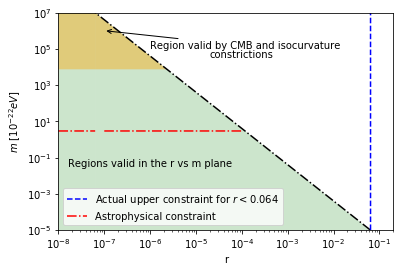
\includegraphics[width=8cm]{SFDMconstraints.png}
\caption{Isocurvature constraints for the SFDM candidate.
\jav{ya me confundio esta figura. Seria bueno poner los ejes al reves, ya que $r$ se esta buscando 
y $m$ seria un derivado. De acuerdo a esta figura, cuales son las constricciones actuales a la masa?}
\jav{quitar la flecha y mejor centrar el texto, explicar regiones.}
}\label{constraintsSFDM}
\end{figure}
%%%%-------------------------------------------------------------------------------------------%%%
%\begin{center}
\subsection{Real Self-interacting SFDM Candidate}
\subsubsection{Cosmological history of a real self-insteracting SFDM particle}
%\end{center}0
%%%-------------------------------------------------------------------------------------------%%%

In this section a self-interacting SFDM with a positive interaction is considered. This scenario is described by the general potentia
\begin{equation}
V(\phi,|\psi|^2)=V(\phi)+\frac{1}{2}m^2\psi^2+\frac{1}{4}\lambda\psi^4.
\end{equation}

Notice that the effective mass of the field is $M^2=m^2+\lambda\psi^2$ \jav{se vale? ya que $\psi$ 
evoluciona, y por tanto la masa también}\lp{Yo le llam ́e masa efectiva,
pero no es realmente una masa}. 
As we have previously discussed the effective mass of the field after inflation remains 
constant at $M^2=m^2+\lambda\psi_i^2$ until $M\sim H$. Then, depending of each contribution to $M^2$, we can 
have two different dynamics. 
\\

%%%-------------------------------------------------------------------------------------------%%%
\textit{Weakly self-interacting regime.-} This limit is obtained when the constant term $m^2$ dominates, 
that is 
%
\begin{equation}\label{consw}
m^2\gg \lambda\psi_i^2.
\end{equation}
In this regime it is possible to ignore the autointeracting term in equation \eqref{KGe3} when the oscillations 
of the scalar field begins. 
However, by ignoring this term the field behaves as a massive field and from
\eqref{rhosfdm} the field value always decreases. Therefore the autointeracting term never dominates and 
all the cosmological history remains the same as in the pure massive SFDM scenario. 

In fact, thanks to the 
decreasing behavior of these scenarios we can consider that this regime is fulfilled always that 
$m^2\geq \lambda|\psi_i|^2/2$ or equivalently when $\lambda\leq 2m^2/|\psi_i|^2$. 
%
If the SFDM oscillations start at the same time than the massive case (which is a good approximation since the effective mass of the SFDM is $M^2 =m^2 +λ\psi^2_i \lesssim 2m^2$), \jav{por que es una buena aproximacion?}\lp{Por lo que agregu\'e en los par\'entesis} we observe from \eqref{phi_im2} that it must be fulfilled that
%
\begin{equation}
\left(\frac{\lambda}{10^{-96}}\right)\leq 1.2\left(\frac{m}{10^{-22}eV}\right)^{5/2}.
\end{equation}
%\jav{estamos hablando del strong or weakly scenario? porq la ecuacion que usas se basa en el weakly scenario!!} 
We plot in figure \ref{weekregime} the weak limit obtained by our approximation. However this overestimates the maximum value of $\lambda$ since the dust-like behavior is obtained when the $\lambda$ term is completely negligible.%
\begin{figure}[h!]
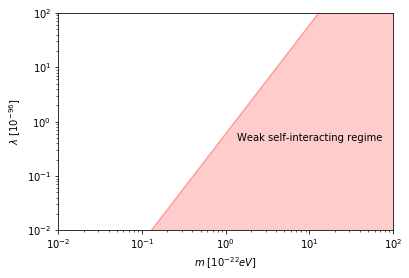
\includegraphics[width=8cm]{weakregime.png}
\caption{Weakly self-interacting regime, \jav{explicar regiones, quitar flecha y mejor centrar el texto}}
\label{weekregime}
\end{figure} 


%%%-------------------------------------------------------------------------------------------%%%
\textit{Strong self-interacting regime.-} This scenario is obtained when 
\begin{equation}
m^2\ll \lambda\psi_i^2.
\end{equation}
%
Here the SFDM follows an attractor solution during the inflationary era, and 
hence within this solution we have two different cases, depending on the attractor solution values.
\\

%%%-------------------------------------------------------------------------------------------%%%
\textit{Attractor behavior of the SF during inflation.-} In the strong self-interacting regime the SFDM follows the 
attractor solution \cite{curvatonatractor}\footnote{The study done in reference \cite{curvatonatractor} was for a curvaton-like model. However their results can be used as well in this context.}
\begin{equation}\label{atractor}
\psi_{att} =\left(2\lambda\int_{\phi}^{\phi_0}V^{-1}_{,\phi}d\phi\right)^{-1/2},
\end{equation}
where $\phi_0$ is the value of the inflaton at the beginning of inflation. 
In the above expression we can identify two possible branches:
\begin{itemize}
\item $\psi_{att}<\sqrt{2}m/\sqrt{\lambda}$

The SFDM follows the attractor solution until $\psi\simeq \sqrt{2}m/\sqrt{\lambda}$. Then the field 
reaches $\psi_i=\sqrt{2}m/\sqrt{\lambda}$ for the rest of inflation. Notice that this value corresponds to the upper 
limit that the weakly self-interacting regime allows. 
%
Then the field starts evolving when $H\sim M\simeq m$ behaving as a massive SF. In this way the constrictions 
given in the non-interacting case apply and the initial conditions are also fixed by $\psi_i$. 
Using both relations the $\lambda$ value is approximated to \jav{la eqn lleva un $\sim$ en lugar de $=$?}\lp{Tienes raz\'on, ya lo cambi\'e}
%
\begin{equation}\label{wregime}
\left(\frac{\lambda}{10^{-96}}\right)\simeq 1.2\left(\frac{g_{*osc}}{3.36}\right)^{3/4}\left(\frac{g_{s*osc}}{3.91}\right)^{-1}\left(\frac{m}{10^{-22}eV}\right)^{5/2}.
\end{equation}
%
The mass term and the auto-interacting constant are rescale by appropriate values, that is, the mass term is measured 
in units of $10^{-22}eV$ while the auto-interacting constant in terms of $10^{-96}$.
\\

\item $\psi_{att}>\sqrt{2}m/\sqrt{\lambda}$

In this scenario the dynamics of the inflaton, given by \eqref{atractor}, implies that the initial condition 
of the field after the inflationary period is
%
\begin{equation}\label{atractor2}
\psi_{att}^i = \left(2\lambda\int_{\phi_{end}}^{\phi_0}V^{-1}_{,\phi}d\phi\right)^{-1/2},
\end{equation}
%
where $\phi_{end}$ is the value of the inflaton at the end of inflation. 
We need to stress out that this is the value of the field until its oscillation period starts (i.e. when $M\sim H$).

In this scenario we observe that at the time the SFDM starts its oscillations its effective mass is quadratic in the field. 
In that regime the scalar field evolves as $\psi\sim 1/a$ and its energy density as $\rho_{\psi}\sim 1/a^4$, 
behaving as radiation. Then, when $m^2 \sim \lambda\psi_t^2$ the effective scalar field mass is now constant, 
obtaining the dust-like behavior already analyzed. 
Therefore, the history of the scalar field density is
%
\begin{equation}\label{rhosfdmlam}
\rho_\psi = \left\lbrace\begin{array}{ll}
\frac{1}{4}\lambda^2\psi_i^4 & \text{when }H\gg \lambda\psi_i^4 \\
\frac{1}{4}\lambda\psi_i^4\left(\frac{a_{osc}}{a}\right)^4 & \text{when }H_t\leq \lambda\psi_i^4\leq H\\
\frac{1}{2}m^2\psi_t^2\left(\frac{a_t}{a}\right)^3 & \text{when } H\leq m^2\ \text{and}\ \lambda\psi^2<m^2
\end{array}\right .
\end{equation}
%
Here sub-index $t$ means quantities measured at transition between radiation-like to dust-like behavior of the SFDM and
\begin{equation}\label{inilamb}
\psi_i^2=\left[\frac{2m^2}{\lambda}\psi_t^2\right]^{1/2}\left(\frac{a_t}{a_{osc}}\right)^2.
\end{equation}
%
Notice that, for simplicity, we have taken an instantaneous transition between radiation-like to dust-like behaviors. 

%In order to continue it is necessary to specify the value of $a_t$ and $a_s$. 
Since the auto-interacting KG equation cannot be solved exactly we work with approximated 
solutions \jav{y numericamente?}\lp{pongo que s\'i se  podr\'ia,  pero  lo  que  me  interesa  es  obtener  la condici\'on inicial $\psi_i$ del campo escalar y obtenerlo como funci\'on de $\lambda$ y $m$. Se me hace mucho m\'as f\'acil
utilizar estas aproximaciones semianal\'iticas que andar resolviendo muchas veces el campo escalar para diferentes $\lambda$s y $m$s para luego comparar}. By using a pure approximated description of the system,
 \cite{SFphi42} obtained the relation (see its equation 80 and 86 and also \cite{SFphi41})\footnote{The reference \cite{SFphi42} obtained this relation by considering a Universe with only a SFDM content. However the result that we are using here can be used in a Universe with several types of matter contents as they explain in their work.} 
 \jav{si ya lo obtuvieron ellos, que obtienes nuevo?}\lp{Hasta  aqu\'i  nada,  s\'olo  estoy usando su resultado para obtener la condici\'on inicial que ando buscando. Tal vez lo nuevo es que yo ya lo estoy mentiendo considerando que el campo escalar coexisti\'o con el inflat\'on, mientras que la referencia que estoy dando lo estudiaron como lo digo en
el pie de p\'agina.}

\lp{Aqu\'i empieza lo que us\'e de Abril y Chavanis}
 %
\begin{subequations}
\begin{equation}\label{atoveras}
\left(\frac{a_t}{a_{osc}}\right)^2=\frac{3}{7^{1/3}f^2(\frac{a_s}{r_S})},
\end{equation}
where 
\begin{equation}
f(\sigma)=\frac{1}{s^{1/3}(1+4s)^{1/6}},
\end{equation}
with
\begin{equation}
s=\frac{4\sigma-1+\sqrt{(4\sigma-1)^2+12\sigma}}{6}.
\end{equation}
\end{subequations}
%
Additionally $r_S=2mG/c^2$ and $a_s=\hbar^2\lambda/4\pi m$. 
Then it follows that $a_s/r_S=\lambda M_p^2/m^2$. 
Rearranging the expression in a more convenient way we have
\begin{equation}
\sigma \simeq 5.93\times 10^{
2}\left(\frac{m}{10^{-22}eV}\right)^{-2}\left(\frac{\lambda}{10^{-96}}\right).
\end{equation}
\lp{Aqu\'i termina}

%
Notice that when $a_t/a_{osc}\simeq 1$ i.e.  $3/(7^{1/3}f^2(\sigma))\sim 1$, there is no radiation-like epoch. 
This scenario should match with the non-interacting scenario that we present previously.  Inserting equation \eqref{atoveras} into \eqref{inilamb} yields to
\begin{equation}\label{inilamb2}
\psi_i^2=\frac{3}{7^{1/3}f^2(\sigma)}\left[\frac{2m^2}{\lambda}\psi_t^2\right]^{1/2}.
\end{equation}
%

The relation (\ref{inilamb2}) matches the field at $\psi_t$ with the value it has right after inflation ends. Then if we obtain the value of $\psi_t$ by comparing with quantities at present, with the above expresion we can also obtain the value of $\psi_i$. On the other hand, notice that at $a_t$ the scalar field behaves as dust with an effective mass $M^2=m^2+\lambda\psi^2_t$. This implies that dust-like oscillations of the SF began a little before than in the non-interacting case. If we allow $m$ to be ultra-light ($m\sim 10^{−22}eV$) and using the fact that $m^2$ is about the same order that $\lambda\psi^2_t$ \jav{de donde se ve esto?}\lp{Anteriormente defin\'i $\psi_t$ como el valor del campo donde se cumple que $m^2\sim \lambda\psi^2_t$} we get that such oscillations start during the same epoch 
than in the non-interacting case. 
%
In fact because the decreasing behavior of the SF at that period \jav{which period}\lp{Cuando comienzas las dust-like oscillations} ($\psi\sim 1/a^{3/2}$) the auto-interacting term contribution quickly vanishes and then the dynamics of the field is described  only by the mass term $m$. Thus, once the dust-like behavior starts, the dynamics 
is described similarly to  the non-interacting case, in such case the condition \eqref{phi_im2} is fulfilled by 
the SF as well, but interchanging subindex $i$ with $t$\footnote{In fact this is a lower limit for the 
strong auto-interacting case.}.
\jav{creo que las ideas estan un poco mezcladas, por que al final siempre terminas con la contribucion $m^2\phi^2$}\lp{Siempre debo terminar con esa contribuci\'on porque al final necesito  que  el  campo  escalar  se  comporte  como polvo.  Entonces lo  \'unico que estoy haciendo aqu\'i es  obtener  cual  es  la  contribuci\'on  de  la  ́\'epoca  de
radiaci\'on.   Digo  que  durante  el  per\'iodo  de  polvo se  cumple  lo  que  ya  hab\'iamos  obtenido  para  un campo masivo y eso lo uso junto con la ecuaci\'on 27 y 28a para obtener la contribuci\'on que da la  \'epoca de radiaci\'on y con ello la condici\'on inicial durante inflaci\'on}
\end{itemize}
%%%=========================================================================%%%
\subsubsection{Constraining isocurvature perturbations for a self-interacting SFDM model}
%%%=========================================================================%%%

As we have shown in the last section we have 2 different scenarios for this model: 
a weak self-interacting and a strong self-interacting. In the weak limit our SFDM behaves 
effectively as a massive field without auto-interaction, and in such case the constrictions 
for the massive field applies to this scenario as well. On the other hand when the auto-interacting 
term is big enough, the SFDM will have a new period with a behavior similar to a radiation-like fluid. 
In this way the constrictions we obtained before will not apply to this model anymore \jav{por que?}
\jav{osea que el weak interacting, no aporta nada?}\lp{El weak interacting es b\'asicamente de nuevo el campo masivo, mientras que en el otro ya tenemos un per\'iodo en el que el SFDM se comporta diferente}.

%Before studying the strong scenario notice that we can give general constrictions for the 
%auto-interacting contribution in terms of our previous expressions. 

In the strong self-interacting regime, during the inflationary era, the SFDM follows the attractor solution \eqref{atractor}.
%\begin{equation}\label{atractor0}
%\psi_{att} =\left(2\lambda\int_{\phi}^{\phi_0}V^{-1}_{,\phi}d\phi\right)^{-1/2}
%\end{equation}
The value that the homogeneous field acquired  after inflation depends on the condition 
$\psi_{att}\lessgtr \sqrt{2}m/\sqrt{\lambda}\equiv \psi_t$. 
For $\psi_{att}<\psi_t$ the field follows the attractor solution until $\psi\simeq \psi_t$. 
Then the SFDM is frozen at that value and starts oscillating as a massive field 
when $m\sim H$. We can constraint this scenario by noticing that it is the same than the massive case but with the initial condition $\psi_i=\psi_t$.  Matching Eq. \eqref{phi_im2} with $\psi_t$ and considering the constriction \eqref{constm} we obtain
%
\begin{equation}
\left(\frac{\lambda}{10^{-96}}\right)\leq 1.2\left(\frac{2\times 10^{-4}}{r}\right)^5.
\end{equation}
In figure \ref{constraintsSFDMl} we have plotted the above condition that is valid in the strong \jav{weak? sure? al inicio del parrafo dice strong}\lp{Me equivoqu\'e, ya lo correg\'i} self-interacting regime when $\psi_{att}<\psi_t$. The  pink  region corresponds with the region allowed by isocurvature perturbations in this limit.  As we can observe the self-interacting term for this model can be constrained in a simmilar way than the mass parameter in the just massive case. This scenario must fulfilled the relation \eqref{constm} as well since its cosmological evolution after inflation is only like a massive SFDM.

\begin{figure}[h!]
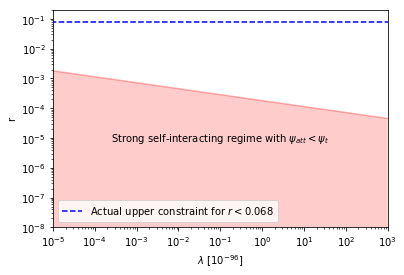
\includegraphics[width=8cm]{lambdavsr.png}
\caption{Isocurvature constraints for the weakly self-interacting term. \jav{weak?}}\label{constraintsSFDMl}
\end{figure} 

Additionally, in this scenario, the inflationary potential fulfills the condition 
%
\begin{equation}
\left(\int^{\phi_0}_\phi V_{,\phi}^{-1}d\phi\right)^{-1/2}<2m.
\end{equation}
%
We can see that it is very difficult to obtain this relation for an ultra-light SFDM candidate. 
For example, if we consider a chaotic-like inflationary potential, $V(\phi)=\frac{1}{2}M_{inf}^2\phi^2$, 
the above conditions implies that
%
\begin{equation}\label{chaoticweek}
\left(\log\frac{\phi_0}{\phi}\right)^{-1/2}<2\frac{m}{M_{inf}}.
\end{equation}
%
However, in a chaotic-like inflationary potential the mass $M_{inf}$ of the inflaton 
that best matches the observations\footnote{This chaotic-like inflationary potential is 
ruled-out now for observations, however we use it as an example in order to obtain 
general constraints for our models.} is of order $M_{inf}\sim 10^{12} GeV$ \cite{Liddle}. 
If now we assume an ultra-light SFDM candidate with a mass $m\sim 10^{-22}eV$, 
the above conditions implies that the logarithmic part of the expression should be 
lower that $\sim 10^{-43}$. The inflationary behavior for a chaotic-like inflaton ends 
when $\phi_{end}\simeq 2M_{pl}$ \cite{curvatonatractor,Liddle}. Moreover as it is 
explained in \cite{curvatonatractor}, the initial condition of the inflaton cannot be 
arbitrarily large since the stochastic behavior is significant for $\dot\phi H^{-1}<H/2\pi$. 
%
If the Universe starts when the inflaton escapes from this 
behavior we have that the initial condition should be
%
\begin{equation}\label{phi_0}
\phi_0\sim 10^5\times M_{pl}\left(\frac{10^{13}GeV}{M_{inf}}\right)^{1/2}.
\end{equation}
%
where we can easily see that the condition given in \eqref{chaoticweek} cannot be fulfilled 
\jav{y si no se satisface, que pasa?}\lp{No podr\'ia estar el campo escalar auto-interactuante en
el r\'egimen d\'ebil con el inflat\'on.  Esto no representa un
gran problema ya que entonces significar\'ia que el campo
escalar deber\'ia estar en el r\'egimen fuerte}. This should implies then that if we consider a self-interacting SFDM candidate coexist with the inflaton it should be in the strong regime since their conditions are easier to be fulfilled.

When $\psi_{att}>\psi_t$ we have that the field follows the attractor solution during all the period of inflation. 
In this way the initial condition for the SFDM is given by \eqref{atractor2}
%
\begin{equation}\label{atractor3}
\psi_{att}^i = \left(2\lambda\int_{\phi_{end}}^{\phi_0}V^{-1}_{,\phi}d\phi\right)^{-1/2}.
\end{equation}
%
Then the SFDM remains frozen at value $\psi_{att}^i$ until $M\sim H$ and starts oscillating with a 
quartic potential. In this scenario the SF density behaves as $\rho_{SFDM}\propto \psi^4$ and 
in such case we can write $\delta\rho_{\psi}/\rho_\psi=4\delta\psi/\psi_i$. In this way the primordial 
isocurvature perturbations for a strong self-interacting SFDM is given by
%
\begin{equation}
P_{SFDM}(k)=\left(\frac{2H_*}{\pi\psi_i}\right)^2.
\end{equation}
%
In the last section we showed the relation of the initial condition  with the value of the 
field today. Using eqs. \eqref{inilamb2} and \eqref{phi_im2}, 
with $g_{*osc}=3.36$ and $g_{s*osc}=3.91$  and considering appropriate units we obtain
%
\begin{equation}\label{constr4}
r<\frac{1.172\times 10^{-4}}{7^{1/3}f^2(\sigma)}\left[\frac{2
\left(\frac{m}{10^{-22}eV}\right)^{3/2}}{\left(\frac{\lambda}{10^{-96}}\right)}\right]^{1/2}.
\end{equation}
%
Similar than in the massive case the above relation must be compared with other constrictions that the strong self-interacting SFDM scenario has. Testing the model at galactic levels by assuming that its ground state 
corresponds with the minimum galaxy halo (Fornax) \cite{SFphi42} it is possible to constraint the ratio $\lambda/m^2$. 
If we use observations coming from the Bullet Cluster \cite{bullet} it is possible to set each of the free parameters of the model \jav{no entendi}\lp{Quiero decir que con FORNAX se obtiene el radio entre $\lambda$ y $m$ y con bullet cluster se fijan los valores que $m$ y $\lambda$ deben tene}. 
In \cite{SFphi42} it was obtained that for a strong self-interacting SFDM model we have
%
\begin{equation}
m\simeq 1.10\times10^{-3}eV, \ \ \ \ \lambda \simeq 2.46\times 10^{-17},
\end{equation}
%
This result corresponds to the upper bound of the mass of the SFDM while the non-interacting case should corresponds with the lower bound. Therefore the mass of the SFDM should be in the range $2.92\times 10^{-22}\lesssim m\lesssim 1.10\times 10^{-3}eV$ while the self-interacting term in the range $0\lesssim \lambda \lesssim 1.69\times 10^{-17}$. On the other hand when the model is tested at cosmological levels using the CMB and the 
abundances of light elements produced by the BBN it is obtained the values \cite{SFphi41,SFphi42}
%
\begin{equation}\label{masslamb}
m\simeq3\times 10^{-21}eV, \ \ \ \ \ \lambda \simeq 1.69\times 10^{-87}.
\end{equation}
%
Notice that these expressions are in agreement with the ones given by galactic constrictions.

Considering \eqref{masslamb} as the most acceptable values for the mass of the SFDM and 
its auto-interacting term we can easily see from Figure \ref{weekregime} that we should be in the strong regime. 
Then in this scenario the constrictions given in Eq. \eqref{constr4} should apply. 

In figure \ref{constraintsSFDMls} we have plotted contour levels of the right side of the relation \eqref{constr4}. The grey region corresponds with values higher than $0.064$ which is the actual upper constraint on tensor-to-scalar ratio. That means that in that region we are certain that \eqref{constr4} is fulfilled and by the momment this region is completely allowed by observations. The white region corresponds with the weak limit. We observe that the parameters obtained by BBN and CMB are easily accepted by the model (red cross) which implies that the isocurvature perturbations are small enough that can avoid actual upper 
constrictions. In this way isocurvature perturbations does not represent any problem for the strong 
self-interacting model that matches with cosmological observations.
%
\begin{figure}
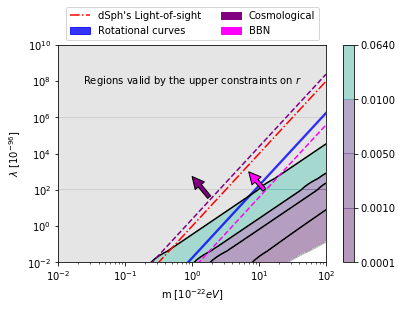
\includegraphics[width=8cm]{stronglamb.png}
\caption{Isocurvature constraints for the strong auto-interacting scenario.
\jav{explicar bien}}\label{constraintsSFDMls}
\end{figure} 

Remark: This scenario is of special interest given that the attractor solution justify the initial 
conditions for the SFDM model and because it is natural to avoid isocurvature perturbations 
when the auto-interacting term of the SF is big enough.
 

Similarly to the above description we can compute general constraints for the inflationary 
potential that should generate inflation on these kind of scenarios. First we have that
%
\begin{equation}
\left(\int^{\phi_0}_\phi V_{,\phi}^{-1}d\phi\right)^{-1/2}>2m,
\end{equation}
%
which is very easy to fulfill as we saw in the chaotic-like example. Using isocurvature constriction we also have
%
\begin{equation}
r<\frac{0.6\times 10^{40}}{\left(\frac{\lambda}{10^{-96}}\right)}\left(\frac{1}{\int_{\phi_{end}}^{\phi_0}V_{,\phi}^{-1}d\phi}\right),
\end{equation}
%
that can also be satisfied as far as the auto-interacting term and the integral are small enough; 
for example in the chaotic-like scenario by using \eqref{chaoticweek} and \eqref{phi_0}
%\begin{equation}
%\left(\int^{\phi_0}_\phi V_{,\phi}^{-1}d\phi\right)^{-1/2}\simeq (0.7403)\times 10^{21}
%\end{equation}
and taking $M_{inf}\simeq 10^{-6}M_{pl} $, we can obtain the constriction 
%
\begin{equation}
\left(\frac{\lambda}{10^{-96}}\right)<\frac{0.3288\times 10^{84}}{r}.
\end{equation}
that is easily satisfied for whichever value of $\lambda$ of our interest.

%
If now we compare \eqref{atractor2} and \eqref{inilamb2} we have
%
\begin{equation}\label{inilamb3}
\left(\int_{\phi_{end}}^{\phi_0}V^{-1}_{,\phi}d\phi\right)^{-1}=\frac{6}{7^{1/3}f^2(\sigma)}\left(2m^2\lambda|\psi_t|^2\right)^{1/2}.
\end{equation}
This relation is interpreted as follows: consider that the auto-interacting SFDM candidate 
coexists with the inflaton, and suppose there are several measurements constraining the mass 
parameter $m$ as well as the auto-interacting parameter $\lambda$, therefore such constraints are translated into 
restrictions to the inflationary potential.  

It is also necessary to be careful that the SFDM does not come to dominate the inflationary period \jav{por que?}\lp{Si domina tendr\'iamos que considerar inflaci\'on
de 2 campos.  Adem\'as tendr\'iamos que justificar como es
que le hizo el campo escalar para luego volverse subdominante y volver a dominar en igualdad materia-radiaci\'on}.  
This is guarantee by demanding that
%
\begin{equation}
\lambda < \frac{H_*^2 M_p^2}{|\psi_i|^4},
\end{equation}
%
or in terms of \eqref{atractor3}
%
\begin{equation}
\lambda>\left(4H_*^2M_{pl}^2\left(\int_{\phi_{end}}^{\phi_0}V_{,\phi}^{-1}d\phi\right)^2\right)^{-1}.
\end{equation}
%
Considering the chaotic-like example and using $H_*= 10^{14} GeV$, we obain the constriction
\begin{equation}\label{lowerlambda}
\frac{\lambda}{10^{-96}} > 5.777\times 10^{77}.
\end{equation}
Notice that the above expresion fulfills astrophysical constrictions but it does not fulfills CMB and BBN. This is not a problem for auto-interacting SFDM models since Eq. \eqref{lowerlambda} is obtained for a 
chaotic-like inflationary potential and, as we already know, that inflationary model is ruled-out by 
the actual constraints given by Planck \lp{Referencia Planck 2018}.



%\begin{center}
%%%-------------------------------------------------------------------------------------------%%%
\subsection{Complex SFDM generalization}
%%%-------------------------------------------------------------------------------------------%%%
%\end{center}
% A massive complex scalar field is described by the potential
%\begin{equation}
%V(|\psi|^2)= m^2|\psi|^2
%\end{equation}
As we have seen at the begining of this section, when we consider a complex scalar field its dynamics is modified 
only by the centrifugal term (see eq. \eqref{KGe3}). However as it was mentioned in \cite{SFphi42} 
such term does not affect the dynamics of the field at cosmological levels, obtaining then that a 
complex scalar field and a real scalar field have the same cosmological history in the Universe. 
%
In this way if we take that our complex SFDM fulfilled slow-roll conditions during inflation then its 
constrictions for isocurvature perturbations must be the same than in the real field analogue. \\

\section{Conclusions}\label{conclusions}
%\begin{center}
%\end{center}


\begin{thebibliography}{9}
\bibitem{const1}  P. A. R. Ade
et al.
(Planck), Astron. Astrophys.
571
, A16 (2014), arXiv:1303.5076 [astro-
ph.CO]
\bibitem{const2} ]  P. A. R. Ade
et al.
(Planck), Astron. Astrophys.
571
, A22 (2014), arXiv:1303.5082 [astro-
ph.CO]
\bibitem{planck} P. A. R. Ade et al. (Planck); DOI: 	10.1051/0004-6361/201525898;  	arXiv:1502.02114 [astro-ph.CO]
\bibitem{SF1} Baldeschi M., Gelmini G., Ruffini R., 1983, Phys.Lett.B, 12
\bibitem{SF2} Matos T., Guzman F. S., 2000, Class. Quant. Grav. 
\bibitem{SF3} Hu W., Barkana R., Gruzinov A., 2000, Physical Review Letters, 85, 1158
\bibitem{SF4}Bray H., 2010
\bibitem{SF5}Schive H.-Y., Chiueh T., Broadhurst T., 2014a, Nature Phys., 10, 496
\bibitem{SF6}B\"ohmer C. G., Harko T., 2007, J. Cosmology Astropart. Phys., 6, 025
\bibitem{SF7}Marsh D. J. E., Ferreira P. G., 2010, Phys. Rev. D, 82, 103528
\bibitem{SF8} Membrado M., Pacheco A. F., Sa\~nudo J., 1989, Phys.Rev.A, 39, 4207
\bibitem{LCDM1}Peebles P. J. E., 1982, ApJ, 263, L1.
\bibitem{LCDM2}White S. D. M., Frenk C. S., Davis M. et al., 1987, ApJ, 313, 505.
\bibitem{problem1}Bullock J. S., Boylan-Kolchin M., 2017, ARA$\&$A, 55, 343
\bibitem{problem2}Clowe D., Bradac M., Gonzalez A. H. et al., 2006, ApJ, 648, 2.
\bibitem{problem3}Klypin A., Kravtsov A. V., Valenzuela O. et al., 1999, ApJ, 522, 82.
\bibitem{problem4}Moore B., Ghigna S., Governato F. et al., 1999, ApJ, 524, L19.
\bibitem{problem5}Penny S., Conselice C. J., De Rijcke S. et al., 2009, MNRAS, 393, 1054.
\bibitem{SF9} J. Maga\~na and T. Matos,  Journal of Physics: Conference Series, Volume 378, conference 1
\bibitem{SF10}  A. Su\'arez, V. H. Robles, and T. Matos, Astrophys. Space
Sci. Proc.
38
, 107 (2014), 1302.0903.
\bibitem{SF11} Marsh D. J. E., 2016, Phys. Rep., 643, 1
\bibitem{SF12}  L. Hui, J. P. Ostriker, S. Tremaine, and E. Witten, Phys. Rev. D
95
, 043541 (2017).
\bibitem{curv1}K. Enqvist and M. S. Sloth, Nucl. Phys. B
626
(2002) 395 doi:10.1016/S0550-3213(02)00043-3
[hep-ph/0109214
\bibitem{curv2} D. H. Lyth and D. Wands, Phys. Lett. B
524
(2002) 5 doi:10.1016/S0370-2693(01)01366-1
[hep-ph/0110002
\bibitem{curv3} T. Moroi and T. Takahashi, Phys. Lett. B
522
(2001) 215 [hep-ph/0110096]
\bibitem{twofields} Christian T. Byrnes, David Wands;  Phys.Rev. D74 (2006) 043529; DOI:  	10.1103/PhysRevD.74.043529;  arXiv:astro-ph/0605679v3
\bibitem{const3}  D. Barkats
et al.
(BICEP1), Astrophys. J.
783
, 67 (2014), arXiv:1310.1422 [astro-ph.C]
\bibitem{const4} P. A. R. Ade
et al.
(BICEP2, Planck), Phys. Rev. Lett.
114
, 101301 (2015), arXiv:1502.00612
[astro-ph.CO]
\bibitem{const5}  P.  A.  R.  Ade
et al.
(BICEP2,   Keck  Array),  Phys.  Rev.  Lett.
116
,  031302  (2016),
arXiv:1510.09217 [astro-ph.CO]
\bibitem{H1}  D. Lyth, Physics Letters B
147
, 403  (1984)
\bibitem{H2}  D. H. Lyth and E. D. Stewart, Physics Letters B
283
, 189  (1992).
%
%
%
% 0
\bibitem{curvaton16} V. Vennin, K. Koyama and D. Wands,
Inflation with an extra light scalar field after Planck
,
JCAP
03
(2016) 024 [
arXiv:1512.03403
] [
IN
SPIRE
].
\bibitem{curvaton15}K.  Enqvist  and  T.  Takahashi,  Journal  of  Cosmology  and  Astroparticle  Physics
2013
,  034
17
(2013),  arXiv:1306.5958.

%
%
%


\bibitem{madelung}  E. Madelung, Zeit. F. Phys.
40
, 322 (1927)
\bibitem{atractorinf1}  V.A.  Belinsky,  L.P.  Grishchuk,  I.M.  Khalatnikov,  and
Ya.B. Zeldovich, Phys. Lett. B
155
, 232 (1985)
\bibitem{atractorinf2}  T.  Piran  and  R.M.  Williams,  Phys.  Lett.  B
163
,  331
(1985)
\bibitem{SFphi41}  B. Li, T. Rindler-Daller, and P.R. Shapiro, Phys. Rev.
D
89
, 083536 (2014)
\bibitem{SFphi42} A. Su\'arez and P. H. Chavanis,
Phys. Rev. D
95
, 063515
(2017)
.
\bibitem{charge1} A. Su\'arez and P.H. Chavanis, Phys. Rev. D
92
, 023510
(2015)
%\bibitem{charge2} \textcolor{red}{ B. Li, T. Rindler-Daller, and P.R. Shapiro, Phys. Rev.
%D
%89
%, 083536 (2014)}
\bibitem{charge3}  A. Arbey, J. Lesgourgues, and P. Salati, Phys. Rev. D
65
, 083514 (2002)
\bibitem{charge4}  J.-A.  Gu  and  W.-Y.P.  Hwang,  Phys.  Lett.  B
517
,
(2001)
  \bibitem{curvatonatractor}   K. Harigaya, M. Ibe, M. Kawasaki and T. T. Yanagida, Phys. Rev. D
87
, 063514
(2013) [arXiv:1211.3535 [hep-ph]].
\bibitem{Planckcolaboration}  P.   A.   R.   Ade
et   al.
[Planck   Collaboration],    Astron.   Astrophys.
594
,    A13   (2016)
[arXiv:1502.01589 [astro-ph.CO]].
\bibitem{SFrev2}T. Kobayashi, R. Murgia, A. De Simone, V. Ir\~si\~c, and M.
Viel,
Phys. Rev. D
96
, 123514 (2017)
.
\bibitem{effdeg}L. Husdal, (2016), 1609.04979.
\bibitem{laldm}L. Visinelli,
Phys. Rev. D 96, 023013 (2017).
\bibitem{massconst1}  P.H. Chavanis, M. Lemou, and F. M ́ehats, Phys. Rev.
D
12
, 123527 (2015)
\bibitem{Liddle}D. H. Lyth and A. R. Liddle, \textit{The primordial density perturbation; cosmology inflation and the origin of structure} , 2009, Cambridge University Press.
\bibitem{bullet}  S.W. Randall, M. Markevitch, D. Clowe, A.H. Gonzalez,
42
and M. Bradac, Astrophys. J.
679
, 1173 (2008)
\bibitem{curvaton9}T. Moroi and T. Takahashi, Phys. Rev. D
66
, 063501 (2002) [arXiv:hep-ph/0206026].
\bibitem{curvaton10}] D. H. Lyth, C. Ungarelli and D. Wands, Phys. Rev. D
67
, 023503 (2003)
[arXiv:astro-ph/0208055]
\bibitem{curvaton11} D. H. Lyth and D. Wands, Phys. Rev. D
68
, 103516 (2003) [arXiv:astro-ph/0306500].
\bibitem{curvaton14} C.  He,  D.  Grin  and  W.  Hu,  Phys.  Rev.  D
92
,  no.  6,
063018 (2015), arXiv:1505.00639.

\bibitem{curvaton4} D. Langlois and F. Vernizzi,
Mixed inflaton and curvaton perturbations
,
Phys. Rev.
D 70
(2004) 063522
[
astro-ph/0403258
] [
IN
SPIRE
].
\bibitem{curvaton5} T. Moroi, T. Takahashi and Y. Toyoda,
Relaxing constraints on inflation models with curvaton
,
Phys. Rev.
D 72
(2005) 023502
[
hep-ph/0501007
] [
IN
SPIRE
\bibitem{curvaton6} T. Moroi and T. Takahashi,
Implications of the curvaton on inflationary cosmology
,
Phys. Rev.
D 72
(2005) 023505
[
astro-ph/0505339
] [
IN
SPIRE
].
\bibitem{curvaton7} K. Ichikawa, T. Suyama, T. Takahashi and M. Yamaguchi,
Non-Gaussianity, Spectral Index
and Tensor Modes in Mixed Inflaton and Curvaton Models
,
Phys. Rev.
D 78
(2008) 023513
[
arXiv:0802.4138
] [
IN
SPIRE
].

\bibitem{curvaton8}T. Suyama, T. Takahashi, M. Yamaguchi and S. Yokoyama,
On Classification of Models of
Large Local-Type Non-Gaussianity
,
JCAP
12
(2010) 030
[
arXiv:1009.1979
] [
IN
SPIRE
].

\bibitem{curvaton3} K. Enqvist and T. Takahashi,
Mixed inflaton and spectator field models after Planck
,
JCAP
10
(2013) 034 [
arXiv:1306.5958
] [
IN
SPIRE
].
\bibitem{curvaton1} A. D. Linde and V. F. Mukhanov, Phys. Rev. D
56
, 535 (1997) [astro-ph/9610219]




%\bibitem{princ_ad}P.J.E. Peebles, \textit{Principle of Physical Cosmology} (Princeton University Press, 1993)
%\bibitem{princ_ad2}A. R. Liddle y S. Lyth, \textit{Cosmological inflation and large scale structure} (Cambridge University Press, 2000).
%\bibitem{curvaton2}D.H. Lyth and D. Wands,
%Generating the curvature perturbation without an inflaton
%,
%Phys. Lett.
%B 524
%(2002) 5.
%[
%hep-ph/0110002
%] [
%IN
%SPIRE
%].
%\bibitem{centrif}  J. A.  Gu  and  W.-Y.P.  Hwang,  Phys.  Lett.  B
%517, (2001)
%\bibitem{qsm2} T.  Piran  and  R.M.  Williams,  Phys.  Lett.  B
%163
%,  331
%(1985)

%\bibitem{curvaton13}  D.  H.  Lyth  and  D.  Wands,  Phys.Rev.
%D68
%,  103516
%(2003), astro-ph/0306500
\end{thebibliography}
\end{document}

